\documentclass{report}
\usepackage[T1]{fontenc}
\usepackage[utf8]{inputenc}
\usepackage{lmodern}
%\usepackage{hyperref}
\usepackage[portuges,brazilian]{babel}
\usepackage{graphicx}
\usepackage{textcomp}
\usepackage{fullpage}
\usepackage{wrapfig}
\usepackage{float}
\usepackage{listings}
\usepackage{amsmath}
\usepackage{amssymb}
\usepackage{subcaption}
\begin{document}

\newcommand{\HRule}{\rule{\linewidth}{0.5mm}}
\newcommand{\tsize}[1]{(\frac{W}{L})_{#1}}
 

%%%%%%%%%%%%%%%%%%%%%%%%%% START TITLE PAGE %%%%%%%%%%%%%%%%%%%%%%%%5
\begin{titlepage}

\begin{center}


{\LARGE UNIVERSIDADE DE SÃO PAULO\\}
{\LARGE DEPARTAMENTO DE ENGENHARIA ELÉTRICA \\}
{\LARGE ESCOLA DE ENGENHARIA DE SÃO CARLOS\\[4cm]}

\textbf{\large SEL5755 - Sistemas Fuzzy}\\[1cm]
\textbf{\large Prof Dr. Ivan Nunes da Silva}\\[2cm]


% Title
\HRule \\[0.6cm]
{ \huge EPC 6\bfseries }\\[0.6cm]

\HRule \\[2cm]

% Author

\begin{center} \large
\emph{Alunos:}\\
\end{center}

\begin{minipage}{0.4\textwidth}
\begin{flushleft} \large
Isabela R. do Prado \textsc{Rossales}\\
6445435
\end{flushleft}
\end{minipage}
\begin{minipage}{0.4\textwidth}
\begin{flushright} \large
Jonas Rossi \textsc{Dourado}\\
6445442
\end{flushright}
\end{minipage}

\vfill

% Bottom of the page
{\large São Carlos,\\ \today}

\end{center}

\end{titlepage}
%\listoffigures
%\begingroup
%\let\clearpage\relax
%\listoftables
%\endgroup
%%%%%%%%%%%%%%%%%%%%%%%%%% STOP TITLE PAGE %%%%%%%%%%%%%%%%%%%%%%%%5


\newpage

A determinação da pressão interna dentro de uma caldeira pode ser estimada em função
de sua temperatura interna e do volume de água em seu interior. O especialista envolvido com o
processo forneceu alguns dados que foram utilizados para o projeto de um sistema \emph{fuzzy} para
mapear o comportamento existente entre as suas entradas e sua saída. Essas informações são as
seguintes:\\

Variáveis de Entrada:\\
Temperatura: varia de 800°C a 1200°C.\\
Volume: varia de $2m^3$ a $12m^3$ de água.\\

Variável de Saída:\\
Pressão: varia de 4 atm a 12 atm.\\

Após a análise preliminar do problema, o projetista propôs um sistema \emph{fuzzy} para
estimar a saída (pressão), a partir das entradas (temperatura e volume), tendo como formato para
as funções de pertinência os seguintes padrões geométricos:

\begin{figure}[hptb]
\centering
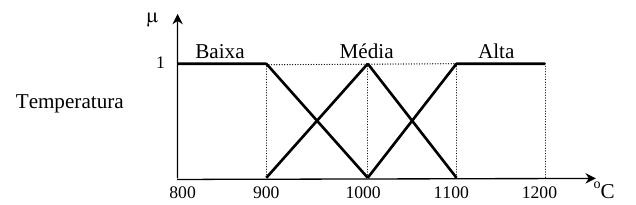
\includegraphics[scale=.8]{g1.png}
\end{figure}

\begin{figure}[hptb]
\centering
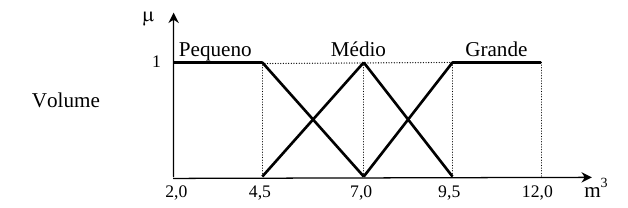
\includegraphics[scale=.8]{g2.png}
\end{figure}

\begin{figure}[hptb]
\centering
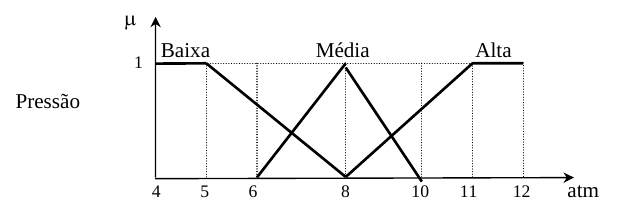
\includegraphics[scale=.8]{g3.png}
\end{figure}


A partir de valores de temperatura e volume, deseja-se então obter valores de pressão.O conjunto de regras
fuzzy é dado pelas seguintes sentenças:\\
Regra 1: \textbf{Se} (Temperatura é Baixa) e (Volume é Pequeno)\\
\textbf{Então} (Pressão é Baixa)\\
Regra 2: \textbf{Se} (Temperatura é Média) e (Volume é Pequeno)\\
\textbf{Então} (Pressão é Baixa)\\
Regra 3: \textbf{Se} (Temperatura é Alta) e (Volume é Pequeno)\\
\textbf{Então} (Pressão é Média)\\
Regra 4: \textbf{Se} (Temperatura é Baixa) e (Volume é Médio)\\
\textbf{Então} (Pressão é Baixa)\\
Regra 5: \textbf{Se} (Temperatura é Média) e (Volume é Médio)\\
\textbf{Então} (Pressão é Média)\\
Regra 6: \textbf{Se} (Temperatura é Alta) e (Volume é Médio)\\
\textbf{Então} (Pressão é Alta)\\
Regra 7: \textbf{Se} (Temperatura é Baixa) e (Volume é Grande)\\
\textbf{Então} (Pressão é Média)\\
Regra 8: \textbf{Se} (Temperatura é Média) e (Volume é Grande)\\
\textbf{Então} (Pressão é Alta)\\
Regra 9: \textbf{Se} (Temperatura é Alta) e (Volume é Grande)\\
\textbf{Então} (Pressão é Alta)\\


\begin{enumerate}

\item[1] Elabore os procedimentos computacionais necessários para obter os valores de saída
(defuzzificados) em função das regiões \emph{fuzzy} resultantes a partir das contribuições de todas as
regras ativadas.

\item[2]  Considere os seguintes valores de temperatura e volume que foram aquisitados em tempo real
pelos instrumentos de medição do processo, os quais são definidos por:

\begin{enumerate}
\item[a)] Temperatura = 965°C e Volume = $11m^3$.
\item[b)] Temperatura = 920°C e Volume = $7.6m^3$
\item[c)] Temperatura = 1050°C e Volume = $6.3m^3$
\item[d)] Temperatura = 843°C e Volume = $8.6m^3$
\item[e)] Temperatura = 1122°C e Volume = $5.2m^3$
\end{enumerate}

Determine, para cada um dos valores acima, quais conjuntos \emph{fuzzy} estarão ativados em função
das entradas (temperatura e volume), listando ainda as respectivas regras \emph{fuzzy} que estarão
associadas com o cálculo da região de saída (pressão) do processo.


\item[3]  Determine e imprima, para cada um dos valores acima, a região \emph{fuzzy} resultante da agregação
de todas as regras ativadas.

\begin{enumerate}
\small
\item[-] Imprima todos os gráficos deste exercício em uma mesma folha.
\item[-] Utilizar 500 pontos de discretização para todos os universos de discurso.
\item[-] Utilizar operador de composição do tipo Max-Min.
\item[-] Utilizar como operador de implicação o operador de Mamdani.
\item[-] Utilizar como operador de agregação o operador Máximo.
\item[-] Utilizar o operador Mínimo para o conectivo “e”.
\end{enumerate}



\item[4]  Baseado nos resultados do Exercício 3, determine então os valores retornados do processo de
defuzzificação quando se aplica o método do “Centro de Área”.


\item[5]  Baseado nos resultados do Exercício 3, determine os valores retornados do processo de
defuzzificação quando se aplica o método da “Média dos Máximos”.


\item[6]  Baseado nos resultados do Exercício 3, determine os valores retornados do processo de
defuzzificação quando se aplica o método do “Primeiro Máximo”.


\end{enumerate}


% \newpage
% 
% Ex. 2 a:
% \begin{figure}[h]
%         \begin{subfigure}[b]{0.6\textwidth}
%                 \centering
%                 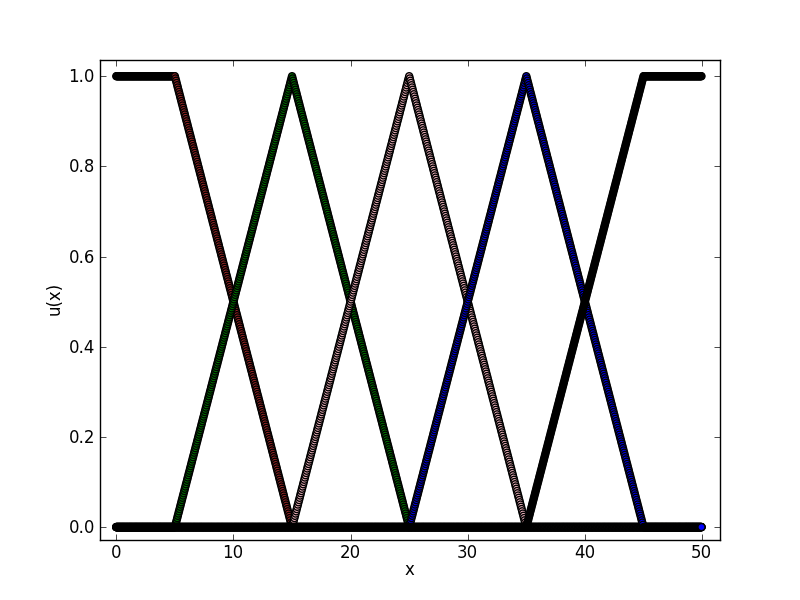
\includegraphics[width=\textwidth]{ex1b1000.png}
% 	\caption{1000 pontos de discretização.}
%         \end{subfigure}
% \end{figure}
% \begin{figure}[h]
% 	\begin{subfigure}[b]{0.6\textwidth}
%                 \centering
%                 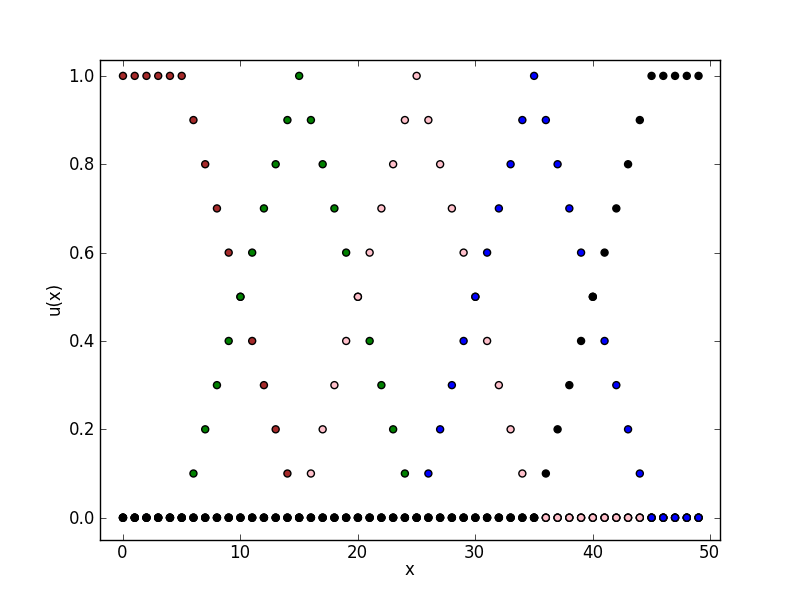
\includegraphics[width=\textwidth]{ex2a50.png}
% 	\caption{50 pontos de discretização.}
% 	\end{subfigure}
% \end{figure}


% \newpage
% Ex. 2 b, c, d:
% 
% \begin{figure}[ht]
%         \begin{subfigure}[b]{0.5\textwidth}
%                 \centering
%                 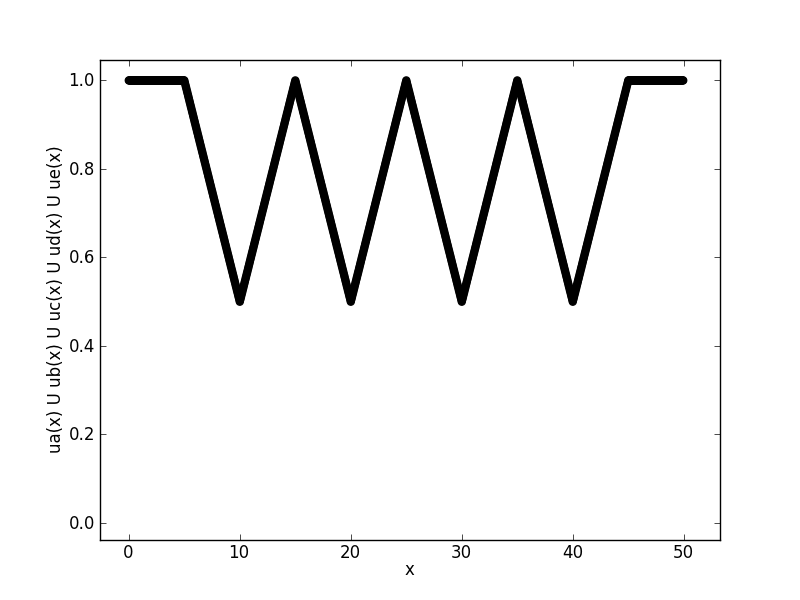
\includegraphics[width=\textwidth]{ex2b.png}
%                 \caption{2b}
%         \end{subfigure}
% 	\begin{subfigure}[b]{0.5\textwidth}
%                 \centering
%                 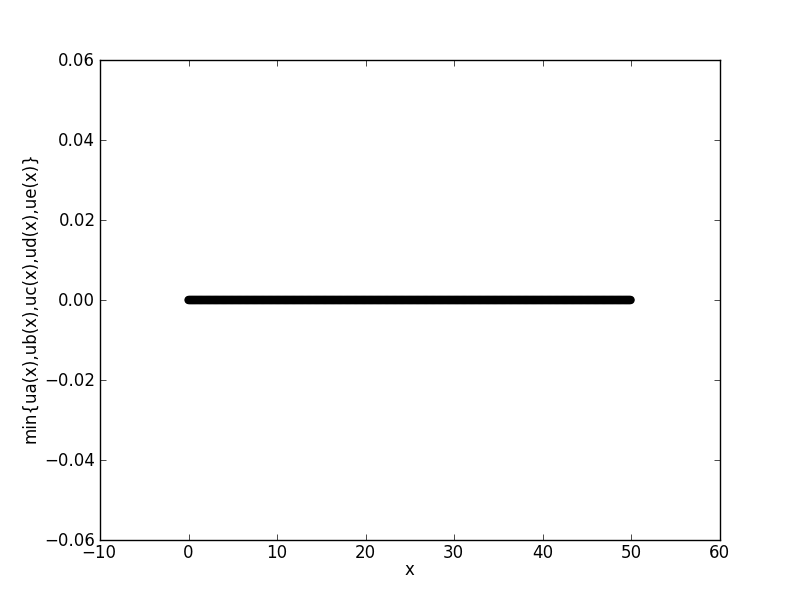
\includegraphics[width=\textwidth]{ex2c.png}
%                 \caption{2c}
% 	\end{subfigure}
% 	\begin{subfigure}[b]{0.5\textwidth}
%                 \centering
%                 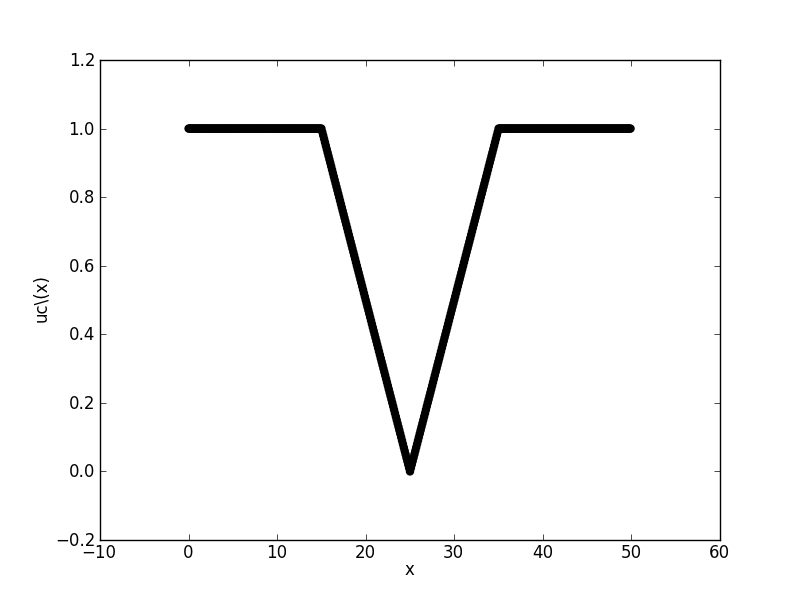
\includegraphics[width=\textwidth]{ex2d.png}
%                 \caption{2d}
% 	\end{subfigure}
% \end{figure}
% 
% 
% \newpage
% 
% Ex. 3:
% \begin{figure}[ht]
%         \begin{subfigure}[b]{0.5\textwidth}
%                 \centering
%                 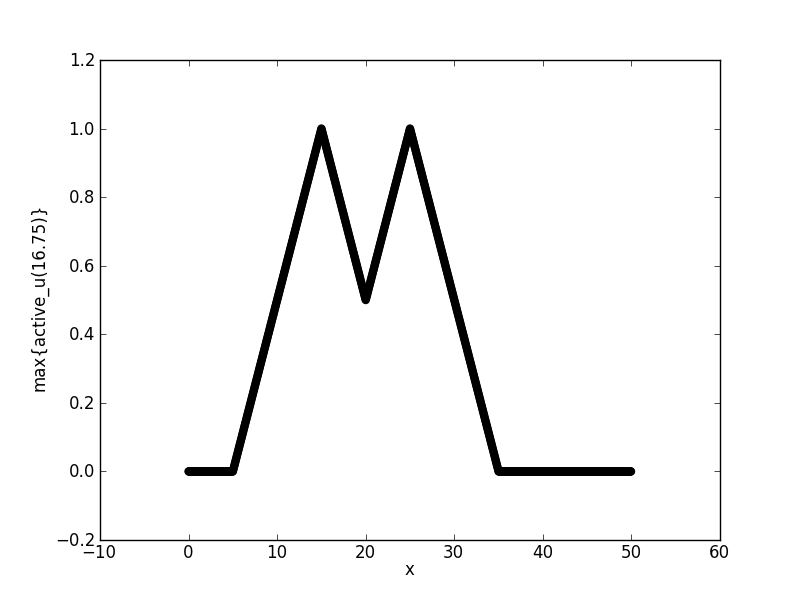
\includegraphics[width=\textwidth]{ex3a.png}
%                 \caption{3a}
%         \end{subfigure}
% 	\begin{subfigure}[b]{0.5\textwidth}
%                 \centering
%                 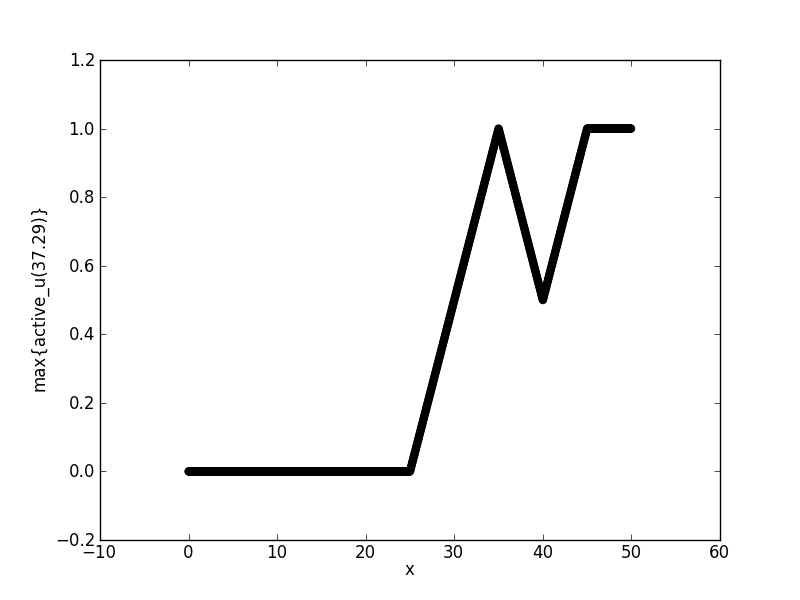
\includegraphics[width=\textwidth]{ex3b.png}
%                 \caption{3b}
% 	\end{subfigure}
% 	\begin{subfigure}[b]{0.5\textwidth}
%                 \centering
%                 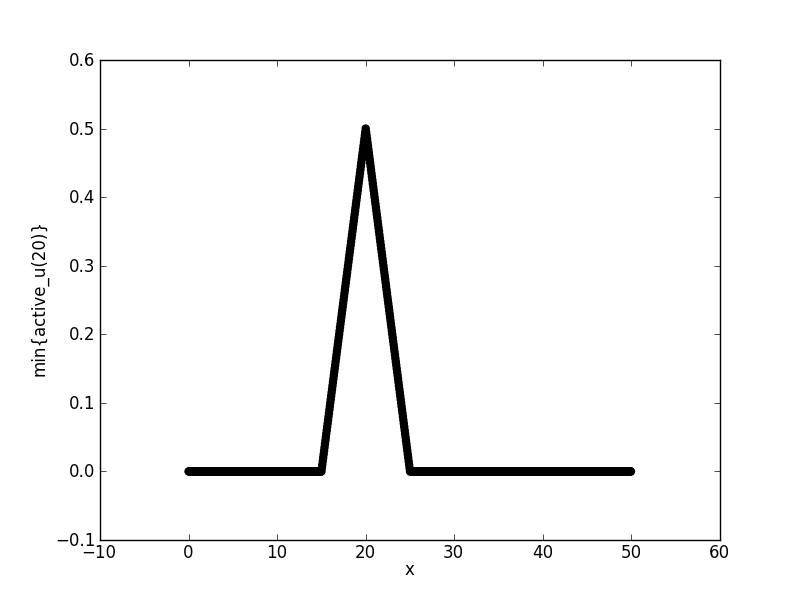
\includegraphics[width=\textwidth]{ex3c.png}
%                 \caption{3c}
% 	\end{subfigure}
% 	\begin{subfigure}[b]{0.5\textwidth}
%                 \centering
%                 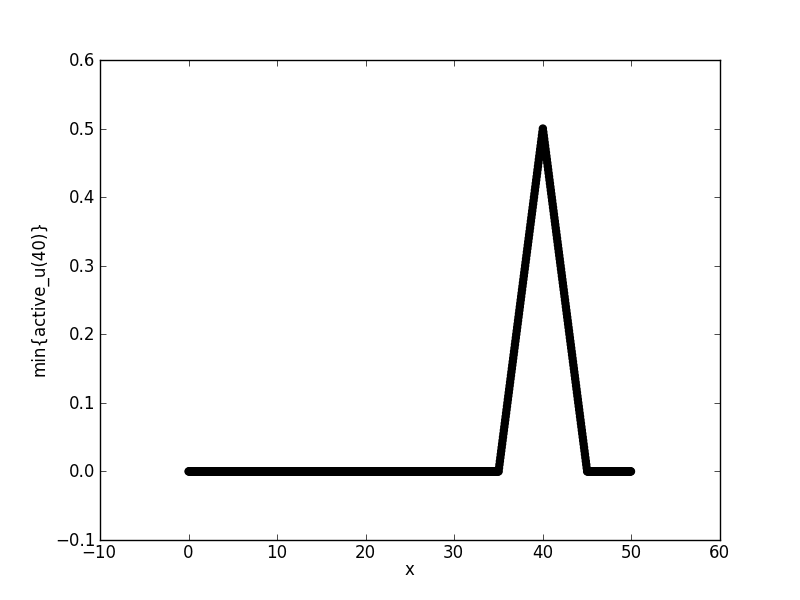
\includegraphics[width=\textwidth]{ex3d.png}
%                 \caption{3d}
% 	\end{subfigure}
% \end{figure}
% 
% 
% \newpage
% 
% Ex. 4:
% \begin{figure}[ht]
%         \begin{subfigure}[b]{0.5\textwidth}
%                 \centering
%                 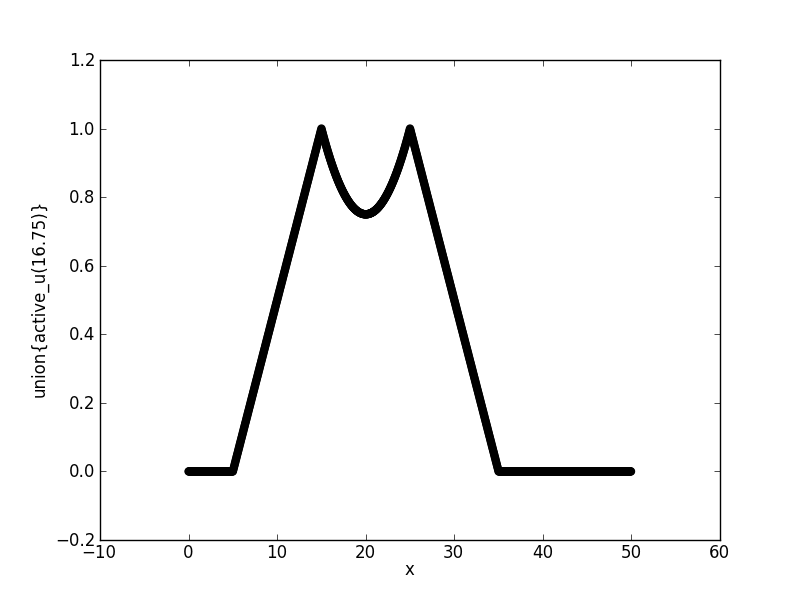
\includegraphics[width=\textwidth]{ex4a.png}
%                 \caption{4a}
%         \end{subfigure}
% 	\begin{subfigure}[b]{0.5\textwidth}
%                 \centering
%                 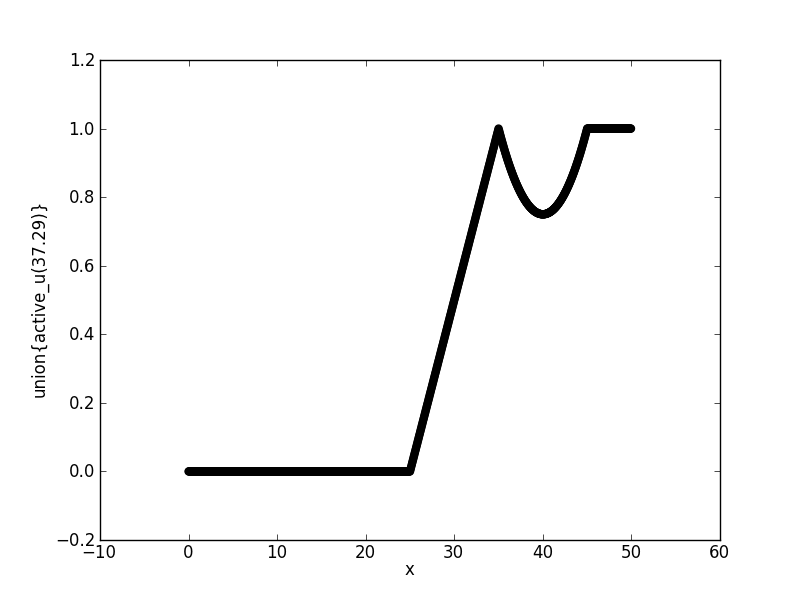
\includegraphics[width=\textwidth]{ex4b.png}
%                 \caption{4b}
% 	\end{subfigure}
% 	\begin{subfigure}[b]{0.5\textwidth}
%                 \centering
%                 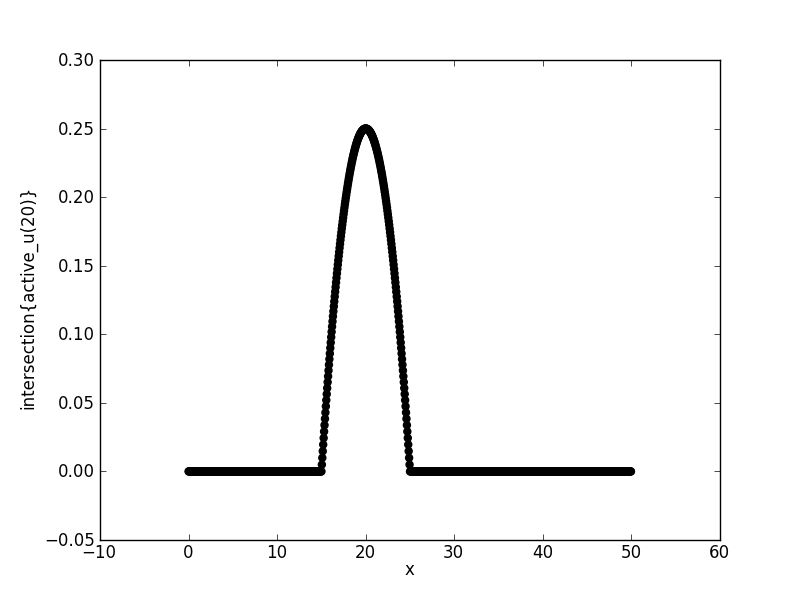
\includegraphics[width=\textwidth]{ex4c.png}
%                 \caption{4c}
% 	\end{subfigure}
% 	\begin{subfigure}[b]{0.5\textwidth}
%                 \centering
%                 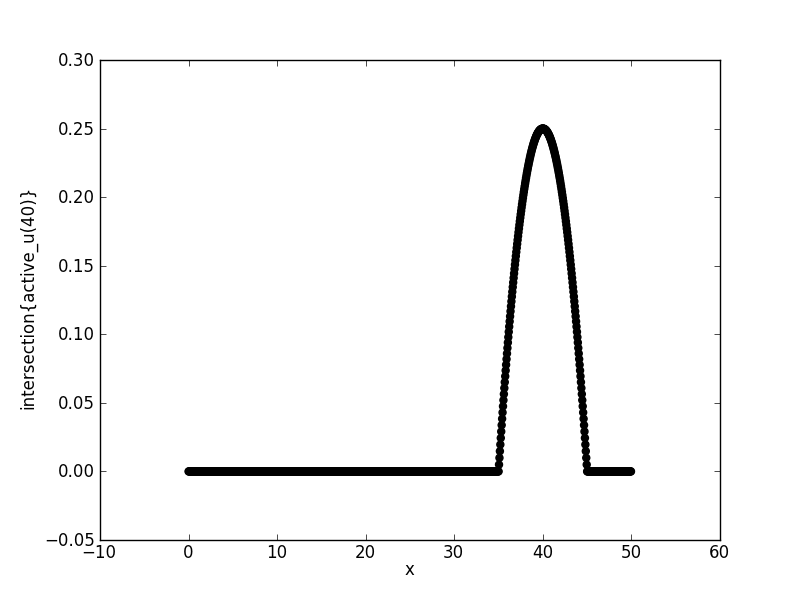
\includegraphics[width=\textwidth]{ex4d.png}
%                 \caption{4d}
% 	\end{subfigure}
% \end{figure}
% 
% 
% \newpage
% Ex. 5:
% \begin{figure}[ht]
%         \begin{subfigure}[b]{0.5\textwidth}
%                 \centering
%                 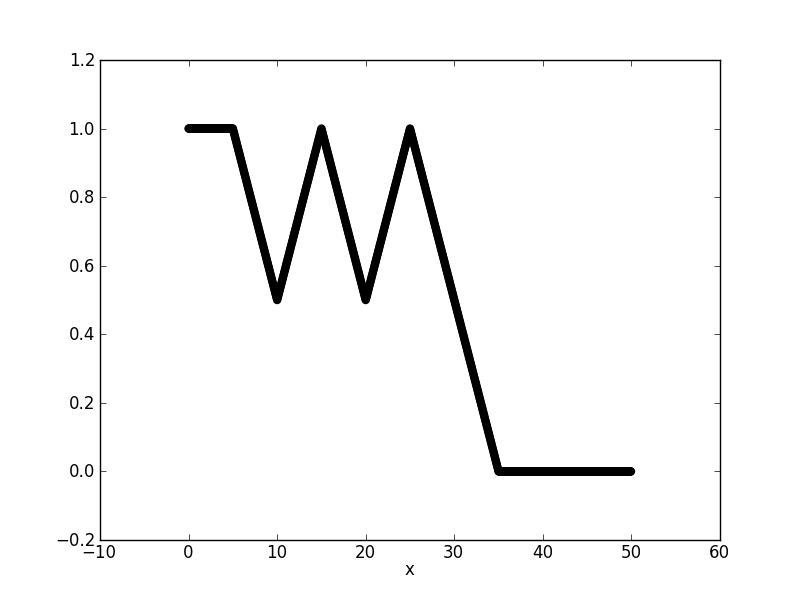
\includegraphics[width=\textwidth]{ex5a.png}
%                 \caption{5a}
%         \end{subfigure}
% 	\begin{subfigure}[b]{0.5\textwidth}
%                 \centering
%                 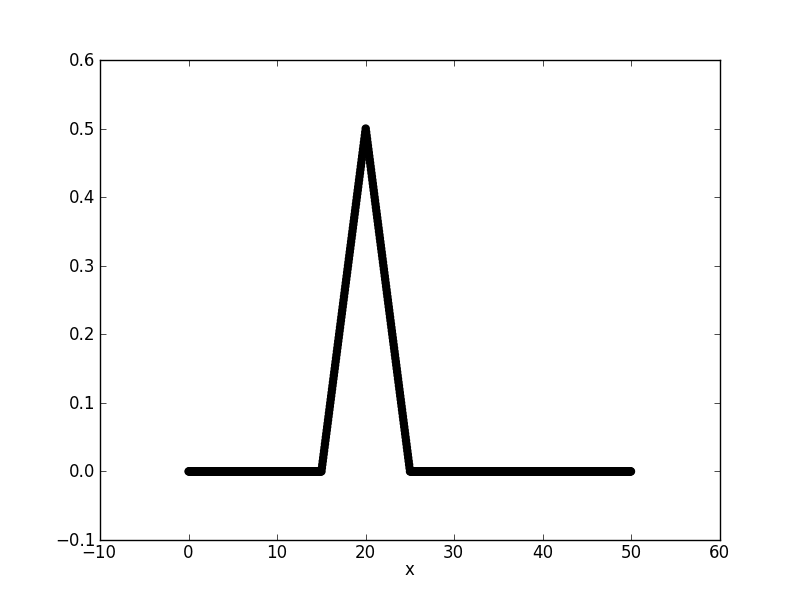
\includegraphics[width=\textwidth]{ex5b.png}
%                 \caption{5b}
% 	\end{subfigure}
% 	\begin{subfigure}[b]{0.5\textwidth}
%                 \centering
%                 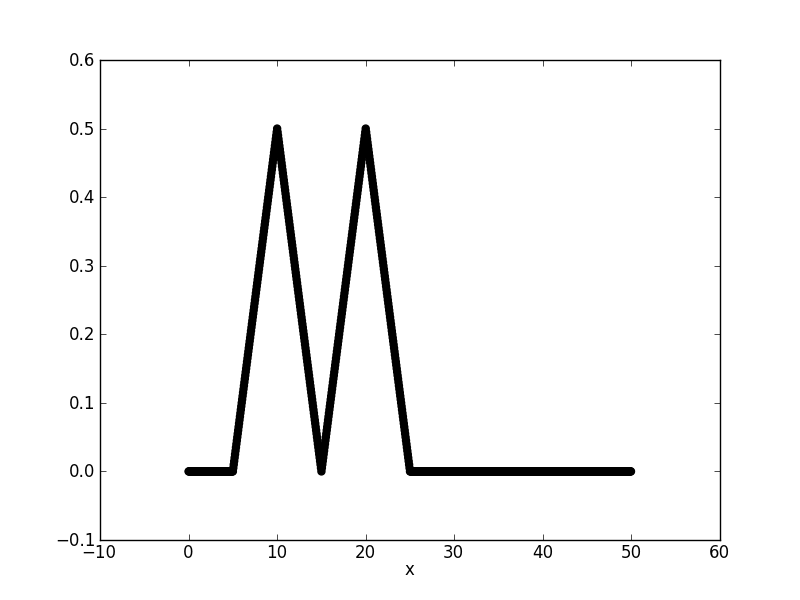
\includegraphics[width=\textwidth]{ex5c.png}
%                 \caption{5c}
% 	\end{subfigure}
% 	\begin{subfigure}[b]{0.5\textwidth}
%                 \centering
%                 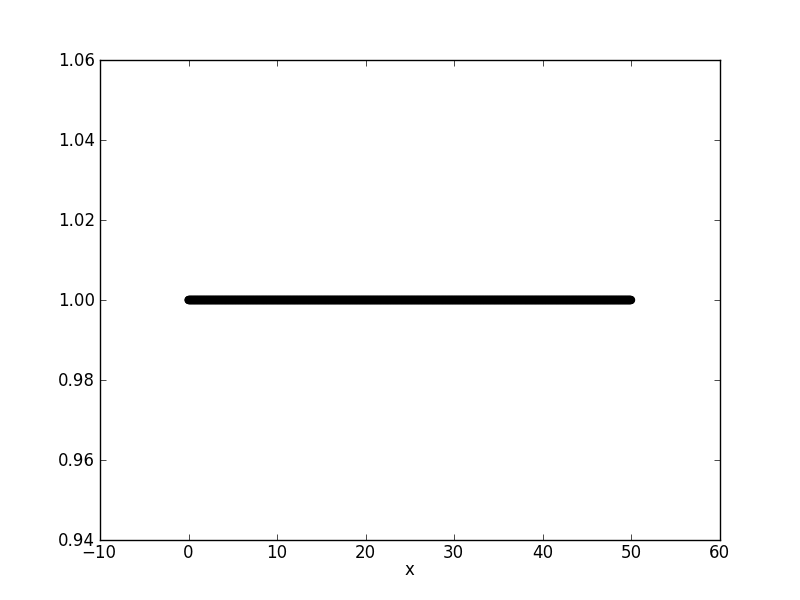
\includegraphics[width=\textwidth]{ex5d.png}
%                 \caption{5d}
% 	\end{subfigure}
% \end{figure}


\newpage
% \lstinputlisting[language=Python]{ex1.py}

\end{document}
